\chapter{The UK Light Injection System}
\label{chp:ukli}

As mentioned in Chapter 4, the Korean laser system is used to measure the scattering and absorbtion coefficients in Super-Kamiokande. The UK calibration group's efforts have been focussed on improving the data analysis method and improving the accuracy of the water coefficient measurements. To aid this effort a new UK developed Light Injection (UKLI) system was installed into Super-Kamiokande during the refurbishment that ocurred in the summer of 2018. The ultimate goal is to install the light injection system in Hyper-Kamiokande, which was the purpose of its initial development. The UK system has its own set of optics, which unlike the Korean system, involves optics with multiple beam spot diameters, which will be described in detail in this Chapter, along with the electronics involved in the production of the system. Much like the Korean laser system method of measuring the absorption and scattering measurements described in Chapter 4, the measurements from the UK system involves the generation of Monte Carlo specific to the diameter of the beam spots produced from the UKLI, the production methods of which will also be discussed in detail in this chapter. Much like for the Korean system, a monitoring system was introduced to observe the light injection output for the different optics, and was also of interest during the Gadolinium loading period to examine changes due to the addition of gadolinium sulphate in the detector. 

\section{The UK Light Injection System Electronics}

The electronics setup architecture for the UK Light Injection system is made of sixteen light emitting diode boards which are each coupled to three optical fibres, as well as a monitor PMT, an optical power meter and two motherboards as shown in Figure \ref{fig:ukli_system_architecture}. 

\begin{figure}
    \centering
    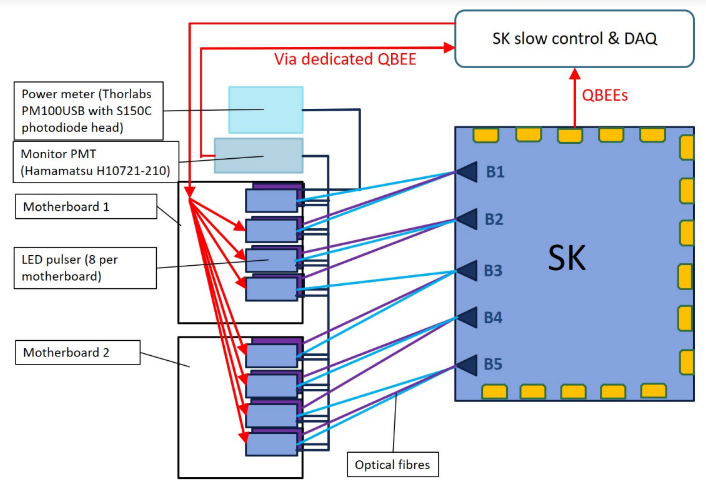
\includegraphics[width=0.7\textwidth]{Figures/ukli_system_architecture.png}
    \caption{UKLI electronics system architecture, showing optical fibre and motherboard couplings and QBEE connections.}
    \label{fig:ukli_system_architecture}
\end{figure}

The light being pulsed has a wavelength of 435 nm and is produced by light emitting diodes which are controlled by Field Programmable Gate Arrays and uses sixteen LED pulser boards placed on two motherboards (8 LED pulser boards on each) which controls which channel to send a signal to. Fifteen of the sixteen channels deliver light into the detector, while the remaining channel sends light to a seperate monitoring system. There are three optical fibres each LED is coupled to: firstly, a channel connected to the monitor PMT, secondly to an optical fibre which sends light into the Super-Kamiokande detector, and finally to the on-board photodiode monitor. The monitor PMT is a very small 2 inch Hamamatsu PMT which has a peak sensitivity to 400 nm wavelength light. A signal is sent from the light emitting diode to the monitor PMT and this information is sent to one of the QBEE (QTC-based electronics with Ethernet) channels for the detector - the charge recorded by the monitor PMT is meant to be used as a normalisation factor for calculations of the absorption and scattering water parameters. 
\newline

The monitor PMT is contained inside a custom made 3D printed box to make sure there is no external light reaching it. There are nineteen channels which monitor the input of the PMT, and these are kept in place against the PMTs photocathode. Fifteen of these fibres are connected to light emitting diodes which give light to the detector, one channel is coupled to the LED board for monitoring the system and the last three channels are reserve. The channel which is coupled to the LED board for monitoring of the syste is used for calibrating the monitor PMT, where the signal from this channel is inputted into the optical power meter. This fibre and the fifteen fibres that are connected to the LEDs that give light to the detector are linked to a photodiode monitor board (PMD). There are two PMDs per motherboard, therefore four in total, which record the output from the LED channels and can switch off a channel if it is producing light when it is not meant to which stops light leaking into the tank. 

\subsection{UKLI System Optics}

Unlike the Korean laser system mentioned in Chapter 4 that injects light into the detector using an optical fibre which has an opening angle of 4 degrees, the UK Light Injection system contains three different types of light injection optics, with each having a different opening angle: a bare fibre, a collimator and a diffuser. This range of optics can accomadate a larger variety of calibration measurements, and better suit the multiple applications of the light injection system, including it being better more monitoring purposes. 

\subsubsection{The Collimator Optic}

A 2-degree opening half angle is achieved by the collimator optic by using a graded index lens (GRIN) connected to a bare fibre optic cable - this GRIN lens reduces the opening angle of the light coming from the fibre optic. A schematic of the collimator design can be seen in Figure \ref{fig:collimator_schematic}. The GRIN lens is kept in position within the lens mount where a HAFC connector is drilled in to take a lens through the centre of the hole inside it, and there is a 2.35 mm diameter opening in front of the glass window in front of the GRIN lens in order to reduce background light which is not on-axis. All holes drilled into the collimator setup are filled with epoxy to prevent water from damaging the components. 

\begin{figure}
    \centering
    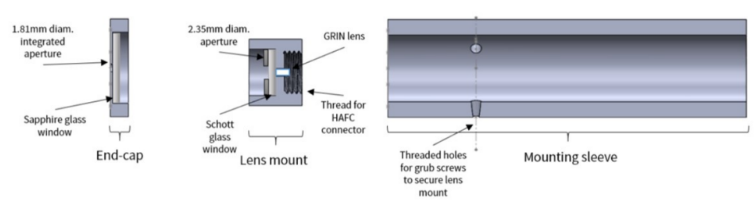
\includegraphics[width=0.7\textwidth]{Figures/collimator_schematic.png}
    \caption{Collimator schematic including the end-cap, lens mount and mounting sleeve structures.}
    \label{fig:collimator_schematic}
\end{figure}

Having such a confined beam allows for a very exact target position on the tank wall, and by decreasing the size of the target beam spot compared to the bare optical fibre, less hit PMTs outside of the target spot are excluded meaning that there are more hits in the water calibration data. Due to the fact that the very collimated beams mean that there is no overlap of beam spots, there can be measurements of the water scattering and absorption coefficients made that are position dependent, allowing for an observation of how the water parameters depend on depth in the tank. 

\subsubsection{The Diffuser Optic}

The diffuser optic is a wide angled beam with a opening half-angle of 40 degrees. It allows for water coefficient measurement calibration and also measurements of PMT gain over time and light attenuation length in water and allows for illumination of several hundred PMTs at once. The diffuser optic is made of a Poly(methyl methacrylate) (PMMA) ball which is a piece of acrylic resin in the shape of a half sphere and it contains PMMA particles suspended in silicone gel, similar to the design of the ''laserball'' used to calibrate the SNO+ detector \cite{Moffat_2005}. As a result of this, the mean free path of light that is injected into the center of the diffuser ball is much shorter than the radius of the ball, so each photon scatters so many times off the PMMA particles at random that the exiting angle of the light is also random. This randomised exit direction of the photons means that the beam timing and intensity would be uniform.  
\newline
The enclosure for the diffuser ball had to be watertight and also able to withstand the pressure of being deployed at the bottom of Super-Kamiokande without the quality of the beam profile being reduced, with the requirement being that it can withstand a maximum pressure of 4 bar. Figure \ref{fig:diffuser_enclosure} shows a photograph of one of the diffusers used, and one of the diffuser ball enclosures. The enclosure is made of high grade stainless steel and using a chemical and water resistant epoxy resin, all the components were ensured to be watertight. 

\begin{figure}
    \centering
    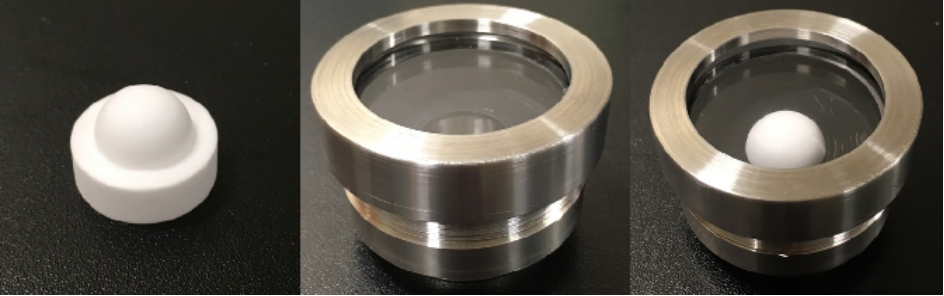
\includegraphics[width=0.7\textwidth]{Figures/diffuser_photo.png}
    \caption{Photograph of the difuser by itself (left), empty diffuser enclosure (centre) and diffuser inside enclosure (right).}
    \label{fig:diffuser_photo}
\end{figure}

\subsubsection{Bare Fibre and Optical Plate}

The bare fibre injector are 1mm step index fibres, and are approximately 20 cm in length and are used for validation purposes with the bare fibres in the Korean optical calibration system. These short fibres are screwed into the back end of the optical plate that the collimator and diffuser optics are mounted on.

Using a kinematic mount (shown in Figure \ref{fig:mount}) the optics plate was attached to the Super-Kamiokande PMT structure - due to the position of the Korean system laser injectors there were two different sizes of optics plates required, as two of the barrel injectors are on a lower PMT rail compared with the other three, meaning that the optical plates on the lower PMT rail include a short piece of metal (known as a ''spacer'') which raises the height of the rail an extra 2.5 inches to remove any interference between the PMTs and the structure.

\subsubsection{Soak Testing Components }

All light injector components that would come into contact with the ultra-pure water in Super-Kamiokande and the gadolinium sulphate doped water went under strenous water contamination testing. Samples of the ultra-pure water were taken from the detector, as well as a control sample of the same water and also a solution of pure water from Super-Kamiokande doped with one gram of gadolinium sulphate and put in 500 ml bottles. The component samples under examination were left to soak in the bottles which were kept refrigerated at the same temperature as the water in Super-Kamiokande (approximately 13 degrees Celcius.) After three months of soaking and intermittent checking of the components by eye, the transmittence of the component (namely the stainless steel used in the optical plate and the PMMA used in the diffuser) were checked using a spectrometer. Comparisons with control components showed no degradation of transmittance. 

